\documentclass[main.tex]{subfiles}
\begin{document}
	Postscript Language Reference, 3rd Edition \cite{PSLF3}
	
	https://www.adobe.com/content/dam/acom/en/devnet/actionscript/articles/PLRM.pdf
	
\begin{figure}[h]
	\centering
	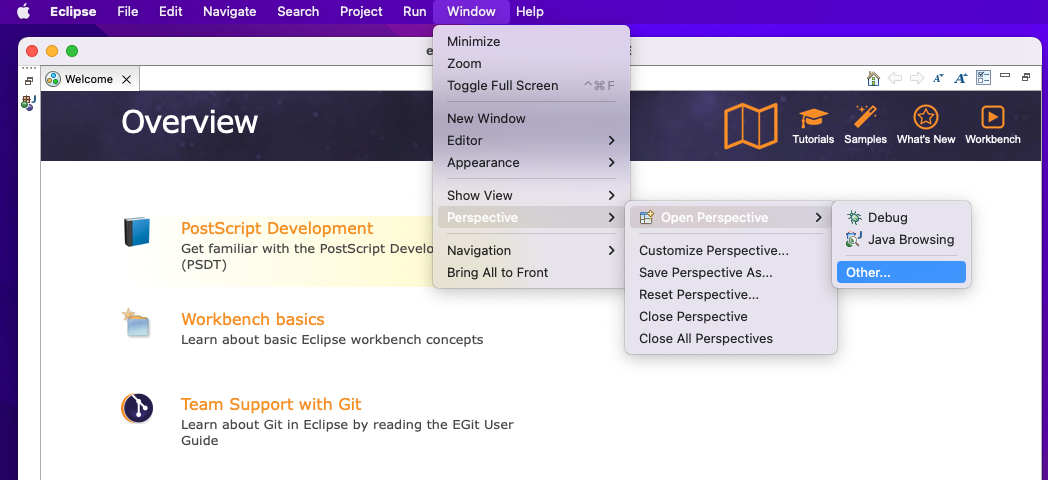
\includegraphics[width=0.95\textwidth]{png/eclipse_perspective}
	\caption{Eclipse Perspective}
	\label{fig:III.1.1}
\end{figure}

\begin{figure}[h]
	\centering
	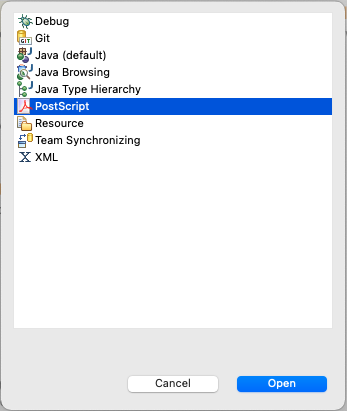
\includegraphics[width=0.5\textwidth]{png/eclipse_perspective_ps}
	\caption{Eclipse Perspective - PostScript}
	\label{fig:III.1.1}
\end{figure}

\begin{figure}[h]
	\centering
	
\includegraphics[width=0.5\textwidth]{images/ps.1.1.eps}
	\caption{$(a+b)^2 = a^2 + 2ab + b^2$}
	\label{fig:III.1.1}
\end{figure}	
	
	
	
\subsection{一些数学公式的几何解释}
$(a+b)^2 = a^2 + 2ab + b^2$


\begin{figure}[h]
    \centering
    
\includegraphics[width=0.5\textwidth]{images/ps.1.1.eps}
    \caption{$(a+b)^2 = a^2 + 2ab + b^2$}
    \label{fig:III.1.1}
\end{figure}

\begin{example} $n$边形的内角和是 $180(n-2)$度, 所以正五边形的内角和是$180\cdot 3 = 540$度,而单个内角则 是$540/5 = 108$度。
\end{example}

\begin{figure}[h]
	\centering
	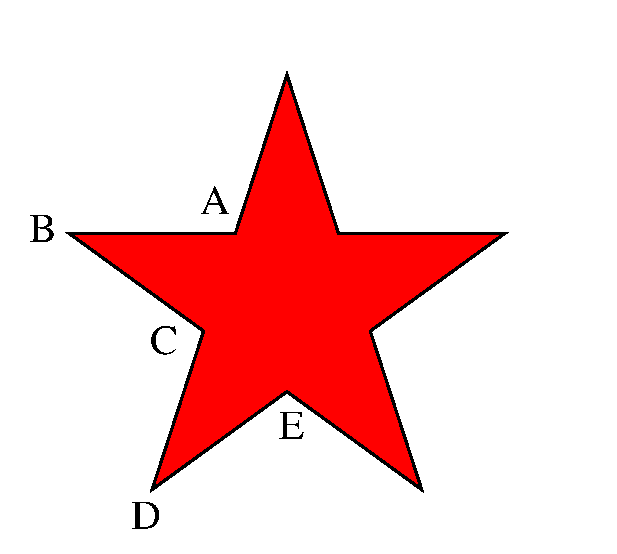
\includegraphics[width=0.5\textwidth]{images/star.eps}
	\caption{红五星}
	\label{fig:III.1.2}
\end{figure}

\begin{figure}[h]
	\centering
	\includegraphics[width=0.5\textwidth]{images/ps/ch_gougu.jpg}
	\caption{《周髀算经》勾股定理图}
	\label{fig:III.1.3}
\end{figure}

\iffalse
\begin{figure}[h]
	\centering
	\includesvg{images/svg/sample}
	\caption{圆盘}
	\label{fig:III.1.3}
\end{figure}
\fi

line spread

line spread
dfdsa;fkadf

\begin{lstlisting}[language=PostScript]
%!PS
/side 80 def %%定义边长 

/angle { %%定义五角星的一个尖角   
 side neg 0 rlineto
 currentpoint translate
-36 rotate
	side 0 rlineto } def

/star {
	newpath
	moveto
	angle  %%先定义一个尖角
	4 { currentpoint translate
		108 rotate
		angle } repeat %%然后靠旋转坐车标系后作出其它四个角色
	closepath } def

gsave  %%保存原始坐标系统的信息
300 500 star  %%描出五星的轮廓路径
1 0 0 setrgbcolor  %%填充红色
fill %%绘出红五星,然后轮廓路径就消失
grestore

300 500 star %%重要新闻描出五星的轮廓路径
0 setgray %%加黑边
stroke

showpage
\end{lstlisting}




Something
\begin{figure}[h]
	\centering
	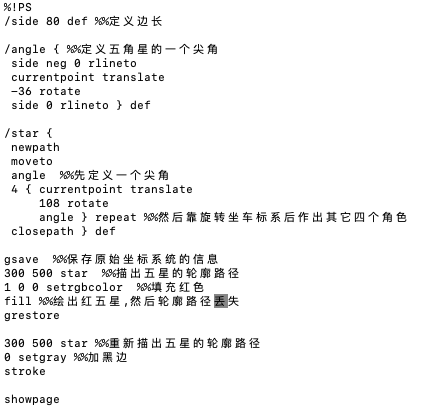
\includegraphics[width=0.5\textwidth]{png/star_code.png}
	\caption{$(a+b)^2 = a^2 + 2ab + b^2$}
	\label{fig:III.1.3}
\end{figure}

\end{document}